\documentclass[11pt,a4paper]{article}
\usepackage[T1]{fontenc}
\usepackage{lmodern}
\usepackage[margin=2.5cm]{geometry}
\usepackage{amsmath,amssymb}
\usepackage{graphicx}
\usepackage{booktabs,tabularx}
\usepackage{microtype}
\usepackage{enumitem}
\usepackage{xurl}
\usepackage[hidelinks]{hyperref}
\usepackage[font=small,labelfont=bf]{caption}
\setlist{nosep,leftmargin=*}
\setlength{\parskip}{0.4em}
\setlength{\parindent}{0pt}
\setlength{\emergencystretch}{2em}
\setlength{\textfloatsep}{12pt}
\setlength{\intextsep}{12pt}
\clubpenalty=10000
\widowpenalty=10000
\brokenpenalty=10000
\renewcommand{\arraystretch}{1.15}

% Author details and all report prose can be edited directly in this file.
\newcommand{\studentname}{Daniyar Ulkhan}
\title{\vspace{-1.2cm}Assignment 5: Clustering and Initialization}
\author{\studentname\\
\normalsize Statistical Methods for Machine Learning, A.Y.\ 2025/26}
\date{}

\begin{document}
\maketitle
\vspace{-0.7cm}

\begin{abstract}
This project compares random initialization and k-means++, two ways of choosing starting centres for k-means. Both use the same clustering loop and were written using NumPy. The experiments use 900 separated synthetic points and 2,000 MNIST digit images. The extensions make the synthetic groups overlap and add noise features which comes up to 784 dimensions. After we run each setting 20 times per method resulting in 320 runs, where both methods reach the same final inertia on the separated data. Random initialization has a slightly lower average inertia and standard deviation on MNIST and the overlapping groups. K-means++ has the lower values in the synthetic 784-dimensional setting. Neither method performs better in every setting.
\end{abstract}

\section{Question and scope}

K-means assigns observations to their nearest centre, which then moves each centre to the average of the group, after it repeats these steps until the groups stop changing. The starting centres at the end will affect the result. And this project asks whether choosing them differently changes the final inertia and makes the results more consistent between runs.

The first method chooses its starting centres uniformly at random from the data. The second uses k-means++ which was proposed by Arthur and Vassilvitskii~\cite{arthur2007}, which gives more weight to observations farther from centres already chosen. After this step both methods use the same Lloyd update loop. The starting rule is the only difference between them.

Following the assignment objectives we use synthetic data with clear groups and a real dataset with several classes and mutliple features. Then we compare inertia and its variation over repeated runs, where for MNIST - the algorithm groups images by their pixel values without using the digit labels. The two extensions examine overlapping groups and extra noise features.

\section{Datasets and evaluation protocol}

\subsection{Synthetic data}

We generate 900 points in two dimensions: 300 around each of the centres $(-5,0)$, $(0,0)$ and $(5,0)$. Both coordinates use independent Gaussian noise with standard deviation $0.7$. Seed 42 makes the generated points repeatable.

The result is three separated clouds, which are shown on the left of Figure~\ref{fig:synthetic}. We choose $k=3$ because the data were generated from three groups. Neither method receives the generating centres, both must choose their own starting centres from the 900 points.

\begin{figure}[htbp]
\centering
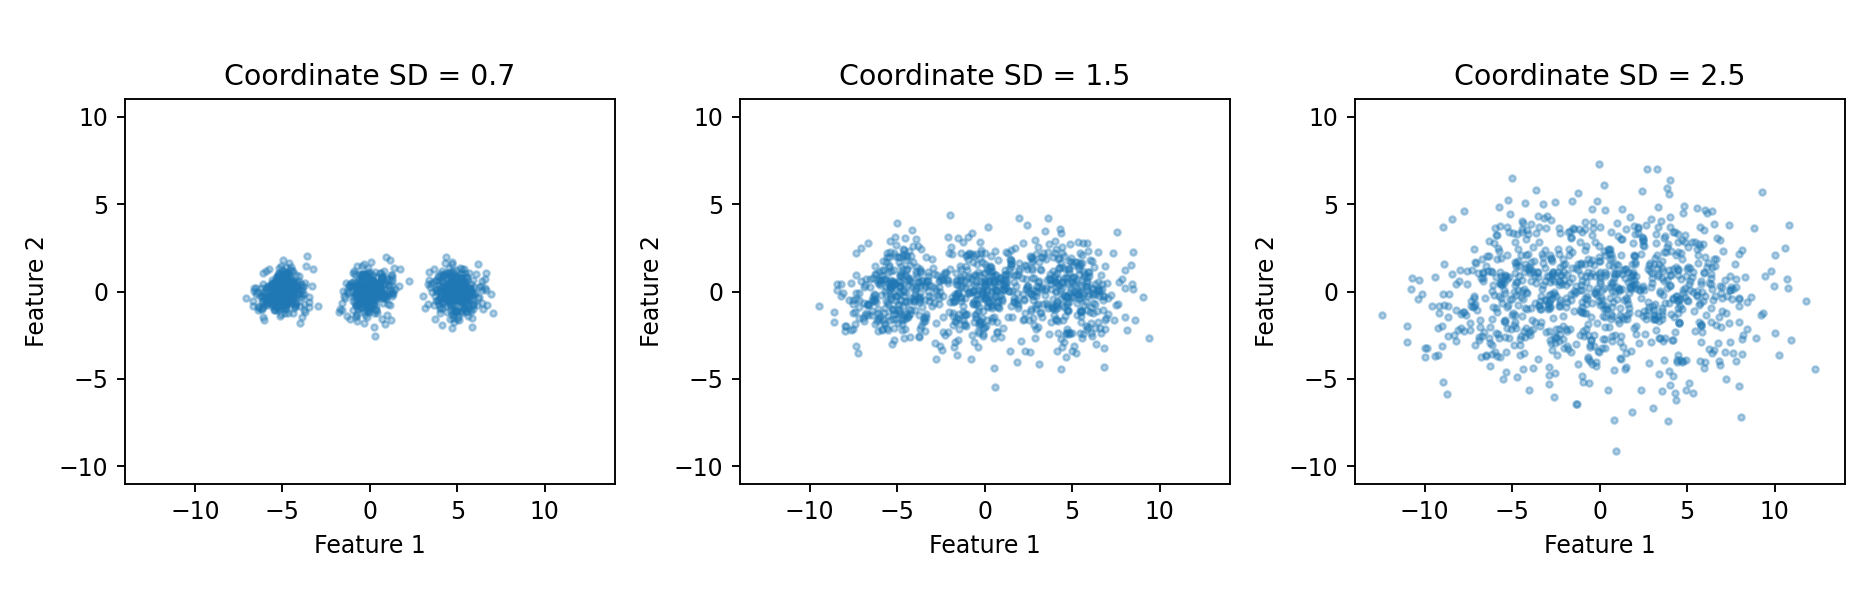
\includegraphics[width=\linewidth]{images/overlap_data.png}
\caption{The synthetic family at coordinate standard deviations $0.7$, $1.5$ and $2.5$, using the same centres and Gaussian offsets. Here the left panel is the original separated dataset and the other panels show increasing overlap. Axes are shared, and the generating centres are not supplied to the algorithms.}
\label{fig:synthetic}
\end{figure}

\subsection{MNIST}

Given MNIST dataset contains images of handwritten digits from 0 to 9. Its training archive has 60,000 images of size $28\times28$ pixels~\cite{mnist}. We then select 2,000 images at random without repeats using seed 42 and ofcourse use this same sample in every run.

As a result each image becomes a row of 784 pixel values. We divide the values by 255 to put them in $[0,1]$. This gives us a dataset with many features, while the smaller sample keeps the repeated runs manageable.

We set $k=10$ since our MNIST dataset contains ten digit categories. Also a cluster is not automatically a digit category: different handwriting styles of the same digit may fall into separate groups, and similar-looking images of different digits may be grouped together to which we have to account.

\begin{figure}[htbp]
\centering
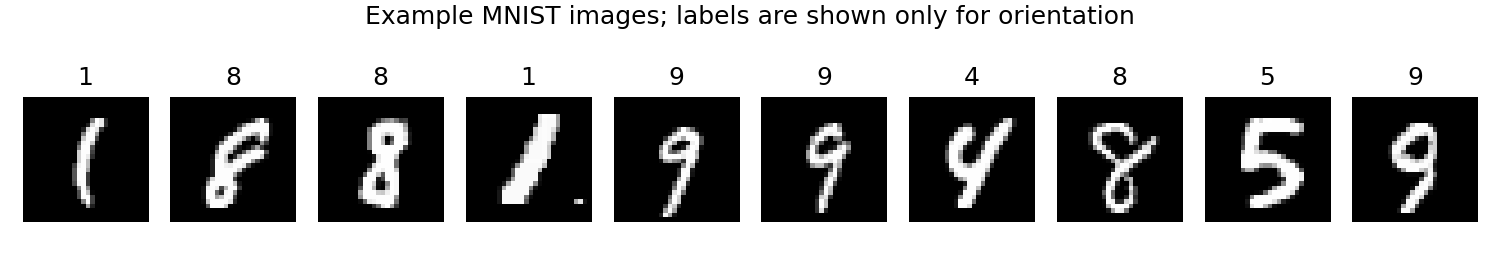
\includegraphics[width=\linewidth]{images/mnist_examples.png}
\caption{The first ten images in the fixed MNIST sample. Labels identify the displayed examples, but are not used by the clustering algorithm.}
\label{fig:mnist}
\end{figure}

The notebook downloads the archive from the location used by Keras and checks its SHA-256 checksum against the official loader source~\cite{loader}. It reads the archive directly, so Keras and TensorFlow are not needed.

\subsection{Overlapping clusters}

For the first extension, we keep the three generating centres, 900 points and $k=3$. We increase the standard deviation from $0.7$ to $1.5$ and $2.5$. The same Gaussian random values generated with seed 42 are scaled to each spread and added to the centres. This makes the groups wider without drawing new random values for every setting. The groups then overlap more, as Figure~\ref{fig:synthetic} shows.

The $0.7$ setting reuses the original synthetic data and its results, and only the other two settings need extra runs. The clustering code is not given the original group labels. Since when we change the spread it also changes the scale of inertia, so we compare the methods at each spread separately.

\subsection{Additional dimensions}

The second extension keeps the original two coordinates and adds independent Gaussian noise features with mean zero and standard deviation $0.7$. The total feature counts are $2$, $10$, $50$, $200$ and $784$. Every setting has 900 points and $k=3$.

We generate the extra features once with seed 43. At each higher feature count, we keep the earlier columns and add more from the same noise matrix. The extra features are generated in the same way for all three groups. This tests what happens when irrelevant information is added to the original data. MNIST is a separate real-data experiment with 784 features.

The two-dimensional results are reused from the original experiment. All spreads, feature counts and run seeds were chosen before the experiments were run.

\subsection{Why the data are kept fixed}

We want to measure the effect of the starting centres and for this reason, every run at a given setting uses the same observations, features and value of $k$. We prepared the synthetic data and MNIST sample only once before the repeated runs.

Afterwards we calculate inertia on the observations being clustered, without a separate training/test split. This lets us compare starting rules on the same data. The MNIST test archive is unused, so these results don't measure performance on new images.

\section{Implementation}

\subsection{Objective and distances}

For observations $x_1,\ldots,x_n$ and centres $c_1,\ldots,c_k$, the objective is
\begin{equation}
J(C)=\sum_{i=1}^{n}\min_{1\leq j\leq k}\lVert x_i-c_j\rVert^2.
\label{eq:inertia}
\end{equation}
This sum is called inertia. With the same data and $k$, so in our case lower inertia means that observations are closer to their group centres.

For MNIST, distance is calculated from the 784 pixel values. Inertia measures how tightly the images are grouped. Its size also depends on the number of observations, number of features and their scale. We therefore compare the methods within each setting.

The function \texttt{squared\_distances} calculates the squared distance from every observation to every centre using
\[
\lVert x-c\rVert^2=\lVert x\rVert^2+\lVert c\rVert^2-2x^\mathsf{T}c.
\]
This formula uses less memory than storing all coordinate differences at once. Any small negative distances caused by rounding are set to zero.

\subsection{Starting centres}

Random initialization chooses $k$ different observations, with each observation equally likely to be selected.

K-means++ chooses the first centre uniformly at random. For each observation, $D_i^2$ is its squared distance to the nearest centre already chosen. The probability of choosing it as the next centre is
\begin{equation}
p_i=\frac{D_i^2}{\sum_{r=1}^{n}D_r^2}.
\label{eq:seeding}
\end{equation}
The distances are updated after each new centre, until $k$ centres are chosen. Observations farther from the existing centres have a greater chance of being selected. The method still makes a random choice and it doesnt always choose the farthest point.

Furthermore observation cannot be selected twice: If all distances are zero, the code chooses another unused observation uniformly at random. This avoids division by zero when the data has duplicate points.

\subsection{Shared update loop}

The function \texttt{fit\_kmeans} uses the following procedure after either initialization:
\begin{enumerate}
\item Assign every observation to its nearest centre.
\item Replace each non-empty cluster centre with the coordinate-wise mean of its assigned observations.
\item Reassign the observations and record the new inertia.
\item Repeat until assignments no longer change, or 200 updates have been completed.
\end{enumerate}

If a cluster is empty the code starts to moves its centre to an observation farthest from its assigned centre. diffrent observations are used if several clusters are empty for these replacements. When distances tie we set the NumPy to consistently choose the first minimum.

Each run returns the centres, assignments, initial and final inertia, inertia history, update count and whether it converged. Both starting methods use the same code. The clustering steps are written using NumPy rather than a ready-made clustering function.

These steps lower inertia or leave it unchanged, apart from rounding error and also our algorithm can still stop when a better clustering exists. As a result 2 runs can converge and finish with different inertia values.

\section{Experimental design}

Table~\ref{tab:design} lists the eight settings. Each has 20 runs per method, using seeds 0 through 19, giving $8\times2\times20=320$ runs. The separated two-dimensional results are shared by the original experiment and both extensions. We run each method once per seed and then save every result.

\begin{table}[htbp]
\centering
\caption{Experimental settings. Each condition uses 20 trials per method and a 200-update cap.}
\label{tab:design}
\small
\begin{tabular}{@{}lrrrr@{}}
\toprule
Conditions & Observations & Features & $k$ & Fits\\
\midrule
Separated synthetic & 900 & 2 & 3 & 40\\
MNIST & 2,000 & 784 & 10 & 40\\
Overlap: $\sigma=1.5,2.5$ & 900 & 2 & 3 & 80\\
Added features: $d=10,50,200,784$ & 900 & 10--784 & 3 & 160\\
\bottomrule
\end{tabular}
\end{table}

The seeds allow the runs to be repeated because the same seed number doesnt give the methods same starting centres, since they choose those centres differently.

We report the mean final inertia, sample standard deviation, minimum and maximum from the 20 runs. The standard deviation uses denominator $20-1$. Relative standard deviation is $100s/\bar{J}$, where $s$ is the sample standard deviation and $\bar{J}$ is mean inertia. It describes the variation as a percentage of the mean.

Here, stability means how much final inertia changes between runs on the same data. We consider it with our mean since consistently reaching a poor score would still give low variation. The code checks that every run converges and that inertia does not increase beyond rounding tolerance. All 320 runs passed and the largest update count was 83, which is below our limit of 200.

\section{Results}

Figure~\ref{fig:distributions} shows the final inertia values, where we can see that each dot is one run. The box covers the middle half of the results, and the line inside marks the median. Small horizontal offsets keep overlapping dots visible. Lower inertia means more compact clusters on the same dataset, while a smaller vertical spread means less variation between runs. We compare the methods within each dataset, since the raw inertia values from different datasets camt be directly compared.

\begin{figure}[htbp]
\centering
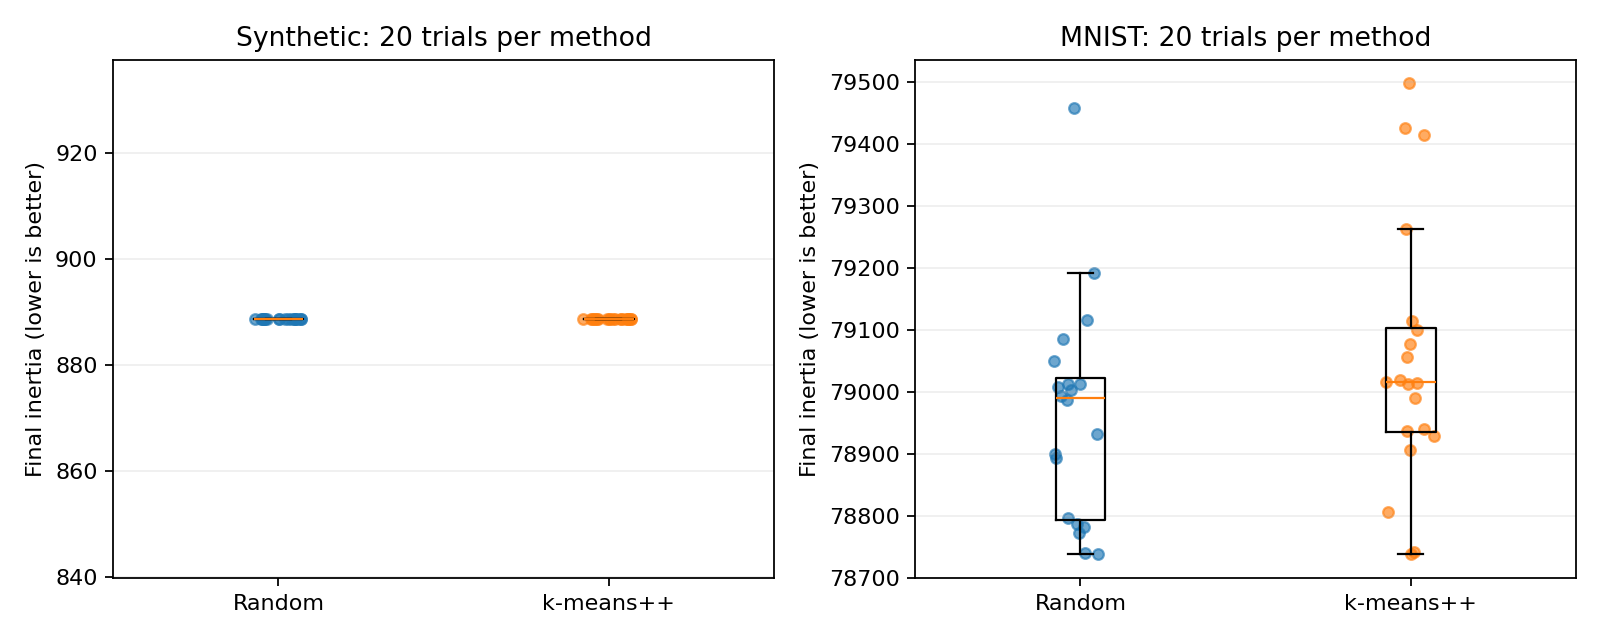
\includegraphics[width=\linewidth]{images/inertia_distributions.png}
\caption{Final inertia over 20 runs per method. The synthetic outcomes are similiar, while the MNIST outcomes vary across seeds. Lower values indicate more compact clusters within a panel.}
\label{fig:distributions}
\end{figure}

\subsection{Synthetic data}

Both methods reached final inertia $888.711$ in every run, to the displayed precision (Table~\ref{tab:synthetic}). The standard deviation is zero, and all 40 runs converged.

The groups are clearly separated and changing the starting centres didn't change final inertia in the runs. As presented neither method had an advantage on this dataset. This agreement doesnt prove that the result is the best possible clustering.

\begin{table}[htbp]
\centering
\caption{Final inertia on the synthetic data, 20 trials per method.}
\label{tab:synthetic}
\begin{tabular}{@{}lrrrr@{}}
\toprule
Initialization & Mean & Sample SD & Minimum & Maximum\\
\midrule
Random & 888.711 & 0.000 & 888.711 & 888.711\\
K-means++ & 888.711 & 0.000 & 888.711 & 888.711\\
\bottomrule
\end{tabular}
\end{table}

\subsection{MNIST}

The MNIST results vary across seeds (Table~\ref{tab:mnist}). Random initialization has mean final inertia $78{,}962.916$, compared with $79{,}049.737$ for k-means++. The difference is $86.821$, or approximately $0.11\%$ of the k-means++ mean.

Random initialization also varied less between runs: its sample standard deviation is $176.468$, compared with $211.037$ for k-means++. It gave slightly tighter groups on average in this experiment. All 40 MNIST runs converged.

\begin{table}[htbp]
\centering
\caption{Final inertia on the fixed MNIST subset, 20 trials per method.}
\label{tab:mnist}
\small
\begin{tabular}{@{}lrrrr@{}}
\toprule
Initialization & Mean & Sample SD & Minimum & Maximum\\
\midrule
Random & 78,962.916 & 176.468 & 78,737.683 & 79,457.876\\
K-means++ & 79,049.737 & 211.037 & 78,737.655 & 79,497.417\\
\bottomrule
\end{tabular}
\end{table}

The best single scores are almost equal: $78{,}737.683$ for random initialization and $78{,}737.655$ for k-means++. Although k-means++ has the slightly better best run, random initialization has the lower average. This is why the comparison includes all runs.

\subsection{Overlapping clusters}

The overlapping groups give small differences between runs (Table~\ref{tab:overlap}). At $\sigma=1.5$, random initialization has mean inertia $3{,}730.362$, compared with $3{,}730.373$ for k-means++. At $\sigma=2.5$, the means are $8{,}665.846$ and $8{,}666.099$. Both differences are below $0.003\%$ of the k-means++ mean. Random initialization also has slightly lower standard deviations.

The relative standard deviations increase from zero at $\sigma=0.7$ to about $0.0061\%$ and $0.0065\%$ at $1.5$, then $0.0157\%$ and $0.0175\%$ at $2.5$, for random initialization and k-means++ respectively. Starting centres therefore make some difference on the overlapping data, but the variation is small. Higher inertia at a wider spread alone does not show that initialization worked worse.

\begin{table}[htbp]
\centering
\caption{Overlap results: mean and sample standard deviation of final inertia. R denotes random initialization; ++ denotes k-means++. Each row uses 20 trials per method.}
\label{tab:overlap}
\small
\begin{tabular}{@{}rrrrr@{}}
\toprule
$\sigma$ & Mean R & Mean ++ & SD R & SD ++\\
\midrule
0.7 & 888.711 & 888.711 & 0.000 & 0.000\\
1.5 & 3,730.362 & 3,730.373 & 0.229 & 0.243\\
2.5 & 8,665.846 & 8,666.099 & 1.362 & 1.517\\
\bottomrule
\end{tabular}
\end{table}

\subsection{Additional irrelevant dimensions}

With $2$, $10$, $50$ and $200$ features, all runs give the same final inertia at each feature count (Table~\ref{tab:dimensions}). At 784 features the k-means++ has mean inertia $344{,}944.397$, compared with $345{,}294.461$ for random initialization whcih are about 0.101\% lower. It also varies less between runs where standard deviation $804.252$ versus $1{,}294.718$. The relative standard deviations are $0.2332\%$ and $0.3750\%$, respectively.

Both methods share the best observed inertia, $344{,}764.151$. Five of the 20 random runs and six of the 20 k-means++ runs reach this value within an absolute tolerance of $10^{-7}$. The other scores produce the difference in mean and spread shown in Table~\ref{tab:dimensions}. K-means++ performed better in this setting, but also other high-dimensional datasets could give different results.

\begin{table}[htbp]
\centering
\caption{Added-feature experiment: mean and sample standard deviation of final inertia. R denotes random initialization; ++ denotes k-means++. Raw inertia is compared within each feature count.}
\label{tab:dimensions}
\small
\begin{tabular}{@{}rrrrr@{}}
\toprule
$d$ & Mean R & Mean ++ & SD R & SD ++\\
\midrule
2 & 888.711 & 888.711 & 0.000 & 0.000\\
10 & 4,338.609 & 4,338.609 & 0.000 & 0.000\\
50 & 21,990.794 & 21,990.794 & 0.000 & 0.000\\
200 & 88,184.207 & 88,184.207 & 0.000 & 0.000\\
784 & 345,294.461 & 344,944.397 & 1,294.718 & 804.252\\
\bottomrule
\end{tabular}
\end{table}

\section{Discussion and limitations}

As a result the difference between methods is minor where both gave the same final inertia on the separated data and after adding features up to 200 dimensions. Random initialization had slightly lower averages on MNIST and the overlapping groups. With 784 synthetic features, k-means++ gave a lower mean and standard deviation. The starting rule therefore mattered more in some experiments than in others: this may be because some datasets have clearer groups than others which leads to similiar results, on opposite when groups overlap there could be many irrelevent features which would make the grouping mudy, and the choice of starting centres has more influence.

Arthur and Vassilvitskii give a bound on the average inertia of k-means++ relative to the best possible clustering~\cite{arthur2007}. This does not promise that it will beat random initialization on every dataset or set of runs. Our mixed results don't contradict that bound.

There are limits to these comparisons. Increasing the spread changes both overlap and the variation inside each group. The extra dimensions do contain noise and we could explore adding useful features that couldve had a different effect. Each setting uses one generated dataset or image sample, fixed $k$ and 20 run seeds. Other samples or cluster counts may give different results

For MNIST, a small change in writing style or stroke position can change pixel distances even when the digit stays the same. Inertia therefore measures how compact the image groups are,so its not a digit-recognition accuracy. We also didn't measure performance on newer observations or running time which could be explored in later iterations. Equal final inertia doesnt mean that all observations have the same assignments.

\section{Conclusion}

Changing the starting centres affected some results more than others. Both methods gave equal final inertia on the separated data and with added features through 200 dimensions. Random initialization had a slightly lower mean inertia and less variation on MNIST and the overlapping groups. K-means++ had the lower mean and variation in our 784-dimensional synthetic experiment, even though both methods reached the same best score.

\begingroup
\small
\begin{thebibliography}{9}
\bibitem{arthur2007}
D. Arthur and S. Vassilvitskii (2007).
\emph{k-means++: The Advantages of Careful Seeding}.
Proceedings of the Eighteenth Annual ACM-SIAM Symposium on Discrete Algorithms (SODA), pp.~1027--1035.
\href{https://research.google/pubs/k-means-the-advantages-of-careful-seeding/}{Publication record}.
\href{https://www.cs.columbia.edu/~verma/classes/uml/ref/clustering_kmean_plusplus_arthur_vassilvitskii.pdf}{Paper copy}.

\bibitem{mnist}
Y. LeCun, C. Cortes and C. J. C. Burges.
\emph{MNIST handwritten digit dataset}.
Dataset description and archive documentation:
\url{https://keras.io/api/datasets/mnist/}.
The documented dataset licence is Creative Commons Attribution-ShareAlike 3.0.

\bibitem{loader}
Keras contributors.
\emph{MNIST dataset loader source}, including the archive URL and checksum.
\url{https://github.com/keras-team/keras/blob/master/keras/src/datasets/mnist.py}.

\bibitem{course}
N. Cesa-Bianchi.
\emph{Statistical Methods for Machine Learning: Experimental Projects},
A.Y.~2025/26, Assignment 5 and general project specifications.
\href{https://docs.google.com/document/d/1JDqx6WXewBjtiyavpbXPFcB4uJ8KG2EhDKwnX-K8xQM/edit}{Course project instructions}.
\end{thebibliography}
\endgroup

\subsection*{Required declaration}

\begin{quote}
\small
I declare that this material, which I now submit for assessment, is entirely my own work and has not been taken from the work of others, save and to the extent that such work has been cited and acknowledged within the text of my work. I understand that plagiarism, collusion, and copying are grave and serious offences in the university and accept the penalties that would be imposed should I engage in plagiarism, collusion or copying. This assignment, or any part of it, has not been previously submitted by me or any other person for assessment on this or any other course of study.
\end{quote}

\end{document}
